%!TEX root = main.tex

\subsection{\textbf{RQ1:} What processes do software developers utilize for merge conflicts?}\label{RQ1}

\begin{figure}[!htbp]
\centering
\fbox{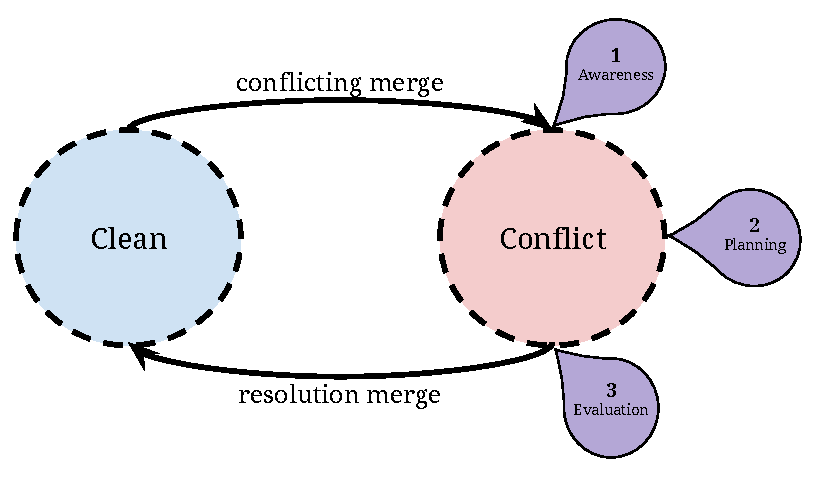
\includegraphics[width=0.98\textwidth,keepaspectratio]{imgs/MergeConflictModel}}
\caption{Model of Developer Processes for Merge Conflicts. Developers alternate between \textit{clean} and \textit{conflicting} states within their codebase. Developers maintain \textit{awareness}~(1) of conflicts within the codebase in different ways. Once aware, developers \textit{plan}~(2) a solution to fix the conflict. And finally, developers \textit{evaluate}~(3) the effectiveness of their deployed resolutions.}
\label{model}
\end{figure}

\begin{itemize}
  \item Results from interviews indicated that a common model of operating with merge conflicts exists.
  \item \textit{Add anecdotal quotes and descriptions from interviews to highlight these observations.}
  \item Based on these anecdotal observations, we construct an initial model of the processes that developers employ when working with merge conflicts, see Fig.~\ref{model}.
  \item To explore and validate this model, we asked developers to reflect upon how they become aware of merge conflicts, how they plan for merge conflict resolutions, and how they evaluate their merge conflict resolutions in the \textit{Processes Survey}~(S1).
  \item We present the results to these research questions in Section~\ref{RQ1a}, \ref{RQ1b}, and \ref{RQ1c}.
\end{itemize}

\subsection{\textbf{RQ1a:} How do software developers become aware of merge conflicts?}\label{RQ1a}

\subsection{\textbf{RQ1b:} How do software developers plan for merge conflict resolutions?}\label{RQ1b}

\subsection{\textbf{RQ1c:} How do software developers evaluate merge conflict resolutions?}\label{RQ1c}